\documentclass[aspectratio=169,12pt]{beamer}
\usepackage{fontspec}
\setmainfont{CMU Serif}
\newfontfamily{\cyrillicfont}{CMU Serif}
\setsansfont{CMU Sans Serif}
\newfontfamily{\cyrillicfontsf}{CMU Sans Serif}
\setmonofont{CMU Typewriter Text}
\newfontfamily{\cyrillicfonttt}{CMU Typewriter Text}

%%% Fonts and language setup.
\usepackage{polyglossia}
%% Math
\usepackage{amsmath, amsfonts, amssymb, amsthm, mathtools} % Advanced math tools.
\usepackage{icomma} % "Умная" запятая: $0,2$ --- число, $0, 2$ --- перечисление

\usepackage{tikz,lipsum,lmodern}
\usepackage[most]{tcolorbox}
\graphicspath{ {images/} }

\usetheme{boxes}
\usecolortheme[style=light]{Nord}
\usefonttheme{Nord}
\setbeamertemplate{navigation symbols}{}%remove navigation symbols
\usepackage{minted}
\usemintedstyle{nord}

\usepackage[dvipsnames]{xcolor}
\usepackage{verbatim}
\usepackage{hyperref}
\usepackage{listings}
\usepackage{tikz,tikz-3dplot}    

\lstdefinelanguage{JavaScript}{
  keywords={let, typeof, new, true, false, catch, function, return, null, catch, switch, var, if, in, while, do, else, case, break},
  ndkeywords={class, export, boolean, throw, implements, import, this},
  identifierstyle=\color{black},
  sensitive=false,
  comment=[l]{//},
  morecomment=[s]{/*}{*/},
  commentstyle=\color{purple}\ttfamily,
  stringstyle=\color{red}\ttfamily,
  morestring=[b]',
  morestring=[b]",
}

\lstset{
  language=JavaScript,
  extendedchars=true,
  basicstyle=\footnotesize\ttfamily,
  showstringspaces=false,
  breakatwhitespace=true,
  showspaces=false,
  numbers=none,
  keepspaces=false,
  breaklines=false,
  showtabs=false,
  captionpos=b
  escapechar =|,
  frame=none,
  commentstyle=\itshape ,
  stringstyle =\bfseries,
  linewidth = \linewidth,
  xleftmargin = -30pt,
  xrightmargin = -15pt,
}

\newtcolorbox{leftBox}{
  colback=NordWhite,colframe=NordBlack, 
  width = 0.97\linewidth,
  sharp corners = southwest,
}

\newtcblisting{rightBox}{
  before=\begin{flushright},
  after=\end{flushright},
  colback=NordWhite,colframe=NordBlack, 
  width = 0.97\linewidth,
  sharp corners = southeast,
  listing only,
}

\setbeamertemplate{footline}[frame number]

%%% Polyglossia setup after  (nearly) everything as described in documentation.
\setdefaultlanguage{russian}
\setotherlanguage{english}

\usepackage{multicol}
\usepackage{xcolor}
\setlength{\columnsep}{0.5cm}

\begin{document}
\begin{frame}
	\begin{center}
		\vspace{1cm}
		\Large\textcolor{NordBrightBlue}{\textbf{Автоматическая генерация фонда оценочных средств ЕГЭ по математике по теме «Стереометрия»}}\\
	\end{center}
	\vspace{0.5cm}
	\large\textcolor{NordBlue}{\textit{Докладчик: Суматохина А.С.}}\\
	\large\textcolor{NordBlue}{\textit{Научный руководитель: д.ф.-м.н., проф. Семенов Е.М.}}\\
	\large\textcolor{NordBlue}{\textit{Научный консультант: асп. Авдеев Н.Н}}\\
	\vspace{0.5cm}
	\begin{center}
		23 апреля 2024 г.
	\end{center}
	\begin{center}
		Воронеж, ВГУ
	\end{center}

\end{frame}

\begin{frame}{Существующие проблемы}
	\begin{itemize}
		%TODO: Тут написан какой-то бред
		\item Дефицит заданий для подготовки
		\item При появлении новых заданий в экзамене — дефицит материалов увеличивается в разы
		\item Списывание ответов учениками
		\item Несоответствие чертежей с условиями задачи
	\end{itemize}
\end{frame}

\begin{frame}{Проект «Час ЕГЭ»}
	\large
	«Час ЕГЭ» — компьютерный образовательный проект, разрабатываемый с 2013~года при математическом факультете ВГУ в рамках «OpenSource кластера» и предназначенный для помощи учащимся старших классов подготовиться к тестовой части единого государственного экзамена
\end{frame}

\begin{frame}{Достижения}
	\begin{multicols}{2}
		\begin{itemize}
			\item Полностью покрыт банк заданий ФИПИ по теме «Планиметрия»
		\end{itemize}
		В ядро добавлены функции для отрисовки:
		\begin{itemize}
			\item Условных обозначений на чертежах, такие как штрих-метка
			\item Углов, в отдельности прямых
			\item Обозначений для равных углов
			\item Отрезков заданной длины под некоторым углом
			\item Строк на середине отрезка
		\end{itemize}
		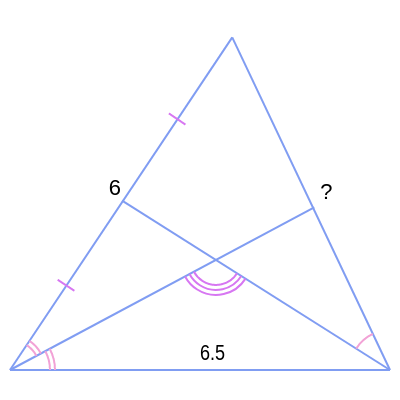
\includegraphics[width=0.9\linewidth]{function_plan.png}
	\end{multicols}
\end{frame}

\begin{frame}{Введение элементов декларативного программирования}
	\textbf{Определение.} Декларативное программирование — парадигма программирования, в которой задается спецификация решения задачи, то есть описывается конечный результат, а не способ его достижения.
\end{frame}

\begin{frame}{Введение элементов декларативного программирования}
	
	\begin{itemize}
		\item Разработано окружение \texttt{retryWhileUndefined} для шаблонов, которое бы перезапускает их не более \texttt{maxIterations} раз, если одно из условий не удовлетворено.
		\item Разработано более совершенное окружение \texttt{retryWhileError}, которое не только могло бы ограничивать количество перезапусков, но и фиксировать, какие проверки не были пройдены и выводить их на экран
	\end{itemize}

\end{frame}

\begin{frame}{Проблема отрисовки многогранников в JavaScript}
	\begin{itemize}
		\item Отсутствуют встроенные средства для изображения трёхмерных фигур
		\item На данный момент существует только одна подходящая библиотека \texttt{Three.js}, которая могла бы выполнить поставленные задачи
		\item При для создания любого объекта необходима не только камера, но и сцена, рендеринг и материал фигуры, что значительно замедляет работу проекта
		\item Другие подобные ей проводят проецирование на плоскость с поворотом только вокруг осей $OX$ и $OZ$
	\end{itemize}
\end{frame}

\begin{frame}{Примеры генерации задач №3}
	\begin{multicols}{2}
		Объём правильной четырёхугольной пирамиды $QRJPZ$ равен $160$ . Точка $V$  – середина ребра  $QR$. Найдите объём треугольной пирамиды  $VRJZ$.\\

		Ответ: $40$

		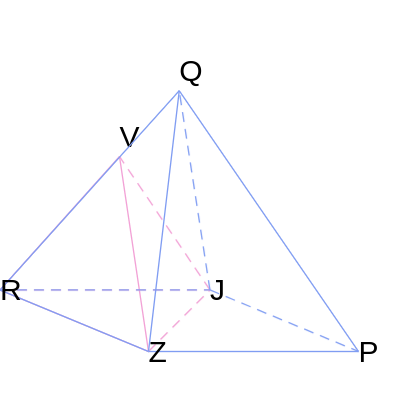
\includegraphics[width=0.4\textwidth]{1.png}
	\end{multicols}

\end{frame}

\begin{frame}{Примеры генерации задач №3}
	\begin{multicols}{2}
		В прямоугольном параллелепипеде           известны длины рёбер: $HA=9$, $HM=3$, $HH_1=14$. Найдите косинус угла между прямыми $H_1M_1$ и $HD$. Ответ умножьте на  $\sqrt{10}$.\\

		Ответ: $1$

		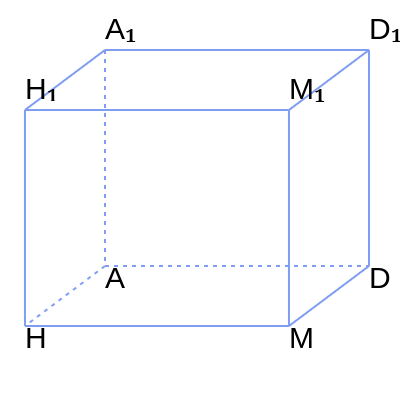
\includegraphics[width=0.4\textwidth]{2.png}
	\end{multicols}

\end{frame}

\begin{frame}[fragile]{Генерация проектора при помощи ChatGPT}
	\begin{leftBox}
		write a 2D to 3D projector in JS without using libraries. input:  point = \{x,y,z\}, camera= \{x,y,z, angleX, angleY, angleZ, scale\}
	\end{leftBox}

	\begin{rightBox}
		function project2Dto3D(point, camera) { ...	return { x: translatedX, y: translatedY, z: translatedZ };
	\end{rightBox}

	\begin{leftBox}
		shorten function project2Dto3D
	\end{leftBox}

	\begin{rightBox}
		function project2Dto3D(point, camera) { ...	return { x: rx + cx, y: ry + cy, z: rz + cz };
	\end{rightBox}
\end{frame}

\begin{frame}{Канонические координаты фигуры}
	\begin{multicols}{2}
		\tdplotsetmaincoords{75}{125}
		\begin{tikzpicture}
			[tdplot_main_coords,
				scale=0.9,
				line/.style={very thick, NordBlue},
				linedash/.style={very thick,dashed, NordBlue},
				diagdash/.style={very thick,dashed, NordBlue},
				axis/.style={->,NordBlack, thick},
				axisdash/.style={thick,dashed, NordBlack},
				figure/.style={opacity=.2,very thick,fill=NordBlue,},]

			\coordinate (O) at (0,0,0);
			\coordinate (A) at (-2,-2,-2);
			\coordinate (B) at (-2,2,-2);
			\coordinate (C) at (2,2,-2);
			\coordinate (D) at (2,-2,-2);

			\coordinate (A1) at (-2,-2,2);
			\coordinate (B1) at (-2,2,2);
			\coordinate (C1) at (2,2,2);
			\coordinate (D1) at (2,-2,2);

			%draw the axes
			\draw[axis] (O) -- (6,0,0) node[anchor=west]{$x$};
			\draw[axis] (O) -- (0,5,0) node[anchor=west]{$y$};
			\draw[axis] (O) -- (0,0,3) node[anchor=west]{$z$};
			\draw[axisdash] (-5,0,0) -- (O);
			\draw[axisdash] (0,-4,0) -- (O);
			\draw[axisdash] (0,0,-3) -- (O);

			%draw the bottom of the cube
			\draw[figure] (A) -- (B) -- (C) -- (D) -- cycle;

			%draw the back-right of the cube
			\draw[figure] (A) -- (B) -- (B1) -- (A1) -- cycle;

			%draw the back-left of the cube
			\draw[figure] (A) -- (D) -- (D1) -- (A1) -- cycle;

			%draw the front-right of the cube
			\draw[figure] (D) -- (C) -- (C1) -- (D1) -- cycle;

			%draw the front-left of the cube
			\draw[figure] (B) -- (C) -- (C1) -- (B1) -- cycle;

			%draw the top of the cube
			\draw[figure] (A1) -- (B1) -- (C1) -- (D1) -- cycle;

			\draw[diagdash] (C) -- (A);
			\draw[diagdash] (B) -- (D);

		\end{tikzpicture}

		\tdplotsetmaincoords{75}{115}
		\begin{tikzpicture}
			[tdplot_main_coords,
				scale=0.9,
				line/.style={very thick, NordBlue},
				linedash/.style={very thick,dashed, NordBlue},
				diagdash/.style={very thick,dashed, NordBlue},
				axis/.style={->,NordBlack, thick},
				axisdash/.style={thick,dashed, NordBlack},
				figure/.style={opacity=.2,very thick,fill=NordBlue,},]

			\coordinate (O) at (0,0,0);

			\coordinate (A) at (3,0,-2);
			\coordinate (B) at (0.9270,2.8531,-2);
			\coordinate (C) at (-2.427,1.7633,-2);
			\coordinate (D) at (-2.4270,-1.7633,-2);
			\coordinate (E) at (0.9270,-2.8531, -2);

			\coordinate (A1) at (3,0,2);
			\coordinate (B1) at (0.9270,2.8531,2);
			\coordinate (C1) at (-2.427,1.7633,2);
			\coordinate (D1) at (-2.4270,-1.7633,2);
			\coordinate (E1) at (0.9270,-2.8531, 2);

			\coordinate (A2) at (-2.43, 0, -2);
			\coordinate (B2) at (-0.75, -2.31,-2);
			\coordinate (C2) at (1.96, -1.43,-2);
			\coordinate (D2) at (1.96, 1.43,-2);
			\coordinate (E2) at (-0.75, 2.31, -2);

			%draw the axes
			\draw[axis] (O) -- (9,0,0) node[anchor=west]{$x$};
			\draw[axis] (O) -- (0,4,0) node[anchor=west]{$y$};
			\draw[axis] (O) -- (0,0,3) node[anchor=west]{$z$};
			\draw[axisdash] (-5,0,0) -- (O);
			\draw[axisdash] (0,-4,0) -- (O);
			\draw[axisdash] (0,0,-3) -- (O);

			\draw[figure] (A) -- (B)  -- (C)  -- (D) -- (E) -- cycle;
			\draw[figure] (A1) -- (B1)  -- (C1)  -- (D1) -- (E1) -- cycle;

			\draw[figure] (A) -- (B)  -- (B1) -- (A1) -- cycle;
			\draw[figure] (C) -- (B)  -- (B1) -- (C1) -- cycle;
			\draw[figure] (D) -- (C)  -- (C1) -- (D1) -- cycle;
			\draw[figure] (D) -- (E)  -- (E1) -- (D1) -- cycle;
			\draw[figure] (A) -- (E)  -- (E1) -- (A1) -- cycle;

			\draw[linedash] (A) -- (A2);
			\draw[linedash] (B) -- (B2);
			\draw[linedash] (C) -- (C2);
			\draw[linedash] (D) -- (D2);
			\draw[linedash] (E) -- (E2);

		\end{tikzpicture}
	\end{multicols}
\end{frame}

\begin{frame}{Этапы генерации}
	\begin{itemize}
		\item Создание объекта нужного класса (фигуры)
		\item Преобразование канонических координат на двумерную плоскость при помощи функции \texttt{project3DTo2D}
		\item Масштабирование координат функцией \texttt{autoScale}
		\item Корректирование матрицы связности (добавление диагоналей или сечений)
		\item Отрисовка фигуры \texttt{drawFigure}
	\end{itemize}

\end{frame}

\begin{frame}{Примеры генерации задач №3}
	\begin{multicols}{4}
		Во сколько раз увеличится объём правильного тетраэдра, если его высота увеличится в $6$ раз?\\

		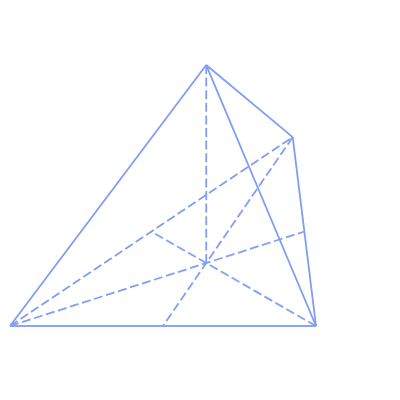
\includegraphics[width=0.3\textwidth]{3}\\

		Во сколько раз увеличится ребро правильного тетраэдра, если его полная площадь поверхности увеличить в $441$ раз?\\

		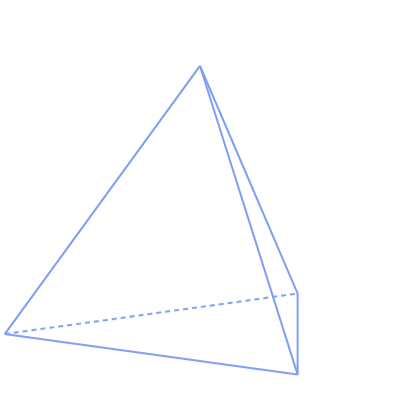
\includegraphics[width=0.3\textwidth]{4}

	\end{multicols}
\end{frame}

\begin{frame}{Примеры генерации задач №3}
	\begin{multicols}{2}
		\footnotesize
		Даны две правильные четырёхугольные пирамиды. Сторона основания первой пирамиды составляет $7$. У второй пирамиды площадь боковой поверхности в $18$ раз больше, а высота в $3$ раза больше, чем у первой. Найдите сторону основания второй пирамиды.\\

		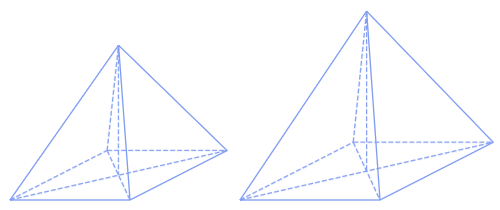
\includegraphics[width=0.5\textwidth]{5}\\
		\vfill\null
		\columnbreak

		Даны две правильные четырёхугольные пирамиды. Сторона основания первой пирамиды составляет $50$ . У второй пирамиды высота в $1.13$  раза больше, а площадь боковой поверхности в $1.6837$  раза больше, чем у первой. Найдите сторону основания второй пирамиды.\\

		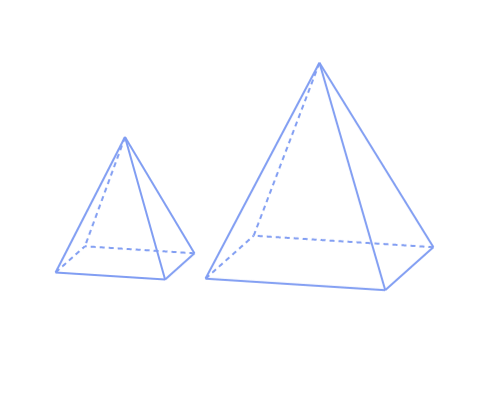
\includegraphics[width=0.5\textwidth,height=4cm]{6}\\

	\end{multicols}
\end{frame}

\begin{frame}{Достижения}
	\begin{itemize}
		\item Полностью покрыт открытый банк заданий ФИПИ по теме «Стереометрия»
		\item Проведён эксперимент по написанию проектора из $\mathbb{R}^3 \to \mathbb{R}^2$ с помощью ChatGPT 3.5 на языке программирования JavaScript
		\item Написана функция отрисовки фигуры на основе её координат и матрицы связности вершин
		\item Написана функция автомасштабирования фигуры
	\end{itemize}

\end{frame}

\begin{frame}{Итоги}
За этот год был полностью покрыт открытый банк заданий ФИПИ по темам:
		      \begin{itemize}
			      \item Планиметрия — 26 шаблонов принято.
			      \item Вектора — 18 шаблонов (10 принято, 8 на внутреннем рецензировании).
			      \item Стереометрия — 56 шаблонов (7 принято, 49 на внутреннем рецензировании).
			      \item Теория вероятности — 10 шаблонов на внутреннем рецензировании.
			      \item Теория вероятности (повышенной сложности) — 11 .шаблонов (1 принят 10 на внутреннем рецензировании).
		      \end{itemize}

В ядро проекта добавлены: 
\begin{itemize}
    \item Функции, упрощающие написание шаблонов по темам «Планиметрия» и  «Стереометрия».
    \item Класс многогранников.
    \item Линейный проектор из $\mathbb{R}^3 \to \mathbb{R}^2$.
\end{itemize}

\end{frame}

\begin{frame}{Итоги}
	\begin{itemize}
		\item Cокращён технический долг проекта
		\item Поставлена цели в будующем добавить в проект класс плоских геометрических фигур и использовать в заданиях по теме «Планиметрия» динамические изображения
\end{itemize}
\end{frame}

\begin{frame}{Список используемых источников}
	\begin{thebibliography}{5}
	\bibitem{chasdok1} Момот Е. А., Арахов Н. Д. Разработка и внедрение ПО для сбора статистики результатов подготовки к ЕГЭ по математике профильного уровня //Актуальные проблемы прикладной математики, информатики и механики. – 2021. – С. 1-2.
	\bibitem{egemath}Открытый банк задач ЕГЭ по математике. Профильный уровень. – URL:  https://prof.mathege.ru/
	\bibitem{fipi}Федеральный институт педагогических измерений. – URL:  https://fipi.ru/ege/otkrytyy-bank-zadaniy-ege
	\bibitem{ege} Единый государственный экзамен. – URL:  https://ru.wikipedia.org/wiki/Единый\_государственный\_экзамен
	\bibitem{sdamgia}Решу ЕГЭ - Сдам ГИА. – URL: https://ege.sdamgia.ru/problem?id=27074
	\bibitem{chas-ege} Тренажёр "Час ЕГЭ". – URL: https://math.vsu.ru/chas-ege/doc/index.html
\end{thebibliography}
\end{frame}

\begin{frame}
	\center\large\textcolor{NordBrightBlue}{\textbf{Спасибо за внимание}}\\
	\hfill \break
	\normalsize
	Все добавленные в проект задания можно сгенерировать по ссылке\\
	\hfill \break

	
\includegraphics[width=0.25\textwidth]{QR-code}\\
	\hfill \break

	\url{https://math.vsu.ru/chas-ege/sh/katalog.html}
\end{frame}

\end{document}
